\chapter{Approach}\label{chap:approach}

\section{Problem Definition}
Sports analytics is, as many previously low-tech markets are, poised to boom as sports organizations are increasingly able to generate more data.  Recent research

\begin{displayquote}
    "The Sports Analytics market is expected to grow from USD 123.7 Million in 2016 to USD 616.7 Million by 2021, at a Compound Annual Growth Rate (CAGR) of 37.9%.

    The increasing volume of on-field and off-field data generated among various sports organizations has led to an increase in managing these data to analyze them. This need is driving the adoption of sports analytics solutions. Analytics and big data technologies have found huge potential in various industries, including sports. The increasing demand of coaches, mentors, and other management officials for real-time access to the insights of relevant information presents huge potential for sports analytics market. The demand for cloud-based sports analytics solutions is also expected to increase due to the lack of budget allocation for hiring technical skills and experts to analyze data for sports organization. These are some of the major factors expected to augment the growth of the market. Moreover, in order to remain competitive, organizations are adopting sports analytics solutions."
\end{displayquote}

\cite{market}

\begin{figure}[!htb]
    \center{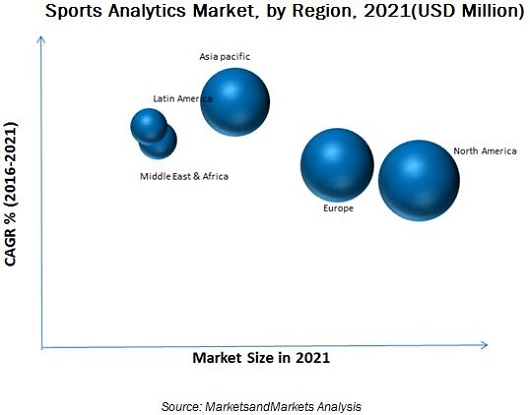
\includegraphics[width=0.4\textwidth]{../figs/sports-analytics-markets.png}}
    \caption{\label{fig:marketsandmarkets} Market Analysis}
\end{figure}
\par
This study was birthed out of a need to reliably quantify three key metrics specifically, each used in assessing a professional basketball player's shooting ability.  Those metris are:


\begin{enumerate}
    \item Odds of making a shot as distance from the basket increases.

    \item Linearity of the decline rate of the probability of making a shot with respect to the distance the shot was taken from the basket.

    \item The relationship between the distance from the shooter to the basket and the odds of the shot being made is different when in the regular season verses the post-season.
\end{enumerate}

Rephrasing those metrics as questions helps clarify the focus of the analysis as it relates to Kobe Bryant. Those questions are as follows:

\begin{enumerate}
    \item Do the odds of Kobe making a shot decrease with respect to distance he is from the hoop?

    \item Does the probability of Kobe making a shot descrease linearly with respect to the distance he is from the hoop?

    \item Is the relationship between the distance Kobe is from the basket and the odds of him making the shot different if they are in the playoffs.
\end{enumerate}

\par
To appropriately answer the questions of interest above, we must fit a series of classifier models to the training portion of our dataset, iteratively scoring and comparing the various models against one another so that we can tune their parameters and hone in on a final feature set.\par
The entirity of the analysis is implemented side-by-side in Python and SAS.
Below, we set the stage for conducting our analysis through an exploratory analysis of the dataset.\par


\section{Exploratory Analysis}

\subsection{Data Overview}
The NBA has provided a comprehensive dataset of every shot Kobe Bryant took throughtout his career.  Accompanying each shot record are a number of supplementary features that provide context to the positioning and environment in which a given shot was taken. Generally, the data was remarkably clean and readily manipulable.  The majority of the wrangling effort was focused on synthesizing new predictors.  A brief summary of the features is below.
\bigbreak
\noindent
\resizebox{\textwidth}{!}{\begin{tabular}{lrrrrrrrr}
    \toprule
    {} &  count &       mean &     std &        min &        25\% &        50\% &        75\% &        max \\
    \midrule
    game\_event\_id     &  25697 &        249 &     150 &          2 &        111 &        253 &        367 &        653 \\
    game\_id           &  25697 &   24741091 & 7738108 &   20000012 &   20500064 &   20900337 &   29600270 &   49900088 \\
    lat               &  25697 &         34 &       0 &         33 &         34 &         34 &         34 &         34 \\
    loc\_x             &  25697 &          7 &     110 &       -250 &        -67 &          0 &         94 &        248 \\
    loc\_y             &  25697 &         91 &      88 &        -44 &          4 &         74 &        160 &        791 \\
    lon               &  25697 &       -118 &       0 &       -119 &       -118 &       -118 &       -118 &       -118 \\
    minutes\_remaining &  25697 &          5 &       3 &          0 &          2 &          5 &          8 &         11 \\
    period            &  25697 &          3 &       1 &          1 &          1 &          3 &          3 &          7 \\
    playoffs          &  25697 &          0 &       0 &          0 &          0 &          0 &          0 &          1 \\
    seconds\_remaining &  25697 &         28 &      18 &          0 &         13 &         28 &         43 &         59 \\
    shot\_distance     &  25697 &         13 &       9 &          0 &          5 &         15 &         21 &         79 \\
    shot\_made\_flag    &  25697 &          0 &       0 &          0 &          0 &          0 &          1 &          1 \\
    team\_id           &  25697 & 1610612747 &       0 & 1610612747 & 1610612747 & 1610612747 & 1610612747 & 1610612747 \\
    shot\_id           &  25697 &      15328 &    8860 &          2 &       7646 &      15336 &      22976 &      30697 \\
    attendance        &  25697 &      15041 &    1076 &      11065 &      14314 &      15048 &      15738 &      20845 \\
    arena\_temp        &  25697 &         70 &       2 &         64 &         69 &         70 &         71 &         79 \\
    avgnoisedb        &  25697 &         95 &       2 &         89 &         93 &         95 &         96 &        102 \\
    \bottomrule
    \end{tabular}}
    \captionof{table}{Feature Summary}\label{tbl:featuresummary}
    \bigbreak

% It is important to note the binary nature of our target feature.

% Please add the following required packages to your document preamble:
% \usepackage{graphicx}
\begin{table}[!hb]
    \centering
    \caption{Key Feature Descriptions}
    \label{my-label}
    \resizebox{\textwidth}{!}{%
    \begin{tabular}{ll}
    Game\_event\_id & Identification variable \\
    Game\_id & Identification variable \\
    Lat and loc\_y & \begin{tabular}[c]{@{}l@{}}Appear to be the same data (y-axis), based on location on the court. \\ The tall bar indicates the frequency of shots taken at the location near the basket\end{tabular} \\
    Loc\_x and lon & \begin{tabular}[c]{@{}l@{}}Appear to be the same data (x-axis), based on location on the court. \\ The tall bar indicates the frequency of shots taken at the location near the basket\end{tabular} \\
    Minutes\_remaining & \begin{tabular}[c]{@{}l@{}}Suggests that there is evidence that Kobe took more shots as the period \\ progressed (higher shot counts closer to the end of the period)\end{tabular} \\
    Period & Indicates similar shot frequency across periods \\
    Playoffs & Playoffs were a rare event in the season, hence the lower shot frequency overall \\
    Season & Shot frequency was lower in 2 seasons \\
    Seconds\_remaining & \begin{tabular}[c]{@{}l@{}}Suggests that there is evidence that Kobe took more shots in the final seconds \\ (higher shot counts closer to the end of the last minute in the period, correlates \\ with shot frequency in the minutes\_remaining variable above)\end{tabular} \\
    Shot\_distance & \begin{tabular}[c]{@{}l@{}}High shot frequency at the basket, at the top of the key (field goals), \\ and the three-point line. Shot frequency was comparatively rarer \\ beyond the three-point line\end{tabular}
    \end{tabular}%
    }
    \end{table}

\par From the available features, the variable "shot\_made\_flag" indicates whether a particular
shot was made (1) or missed (0), and is the feature that acts as our endogenous variable. The remainder of the features are the potential predictors, or exogenous variables. Since there are a managable number of them, we can simply generate descriptive plots for each exogenous feature.  Univariate distribution or frequency plots are ideal for vizualizing the underlying distristribution of each variable. In addition, boxplots for each exogenous feature against each level of the endogenous variable allowed us to develop our intuition about the variance within each level of the target feature.\par

Most of the features show no signs of skewness or severe departures from normality, however, there are some exceptions.



\begin{figure}
    \centering
    \begin{subfigure}[b]{0.4\textwidth}
        \center{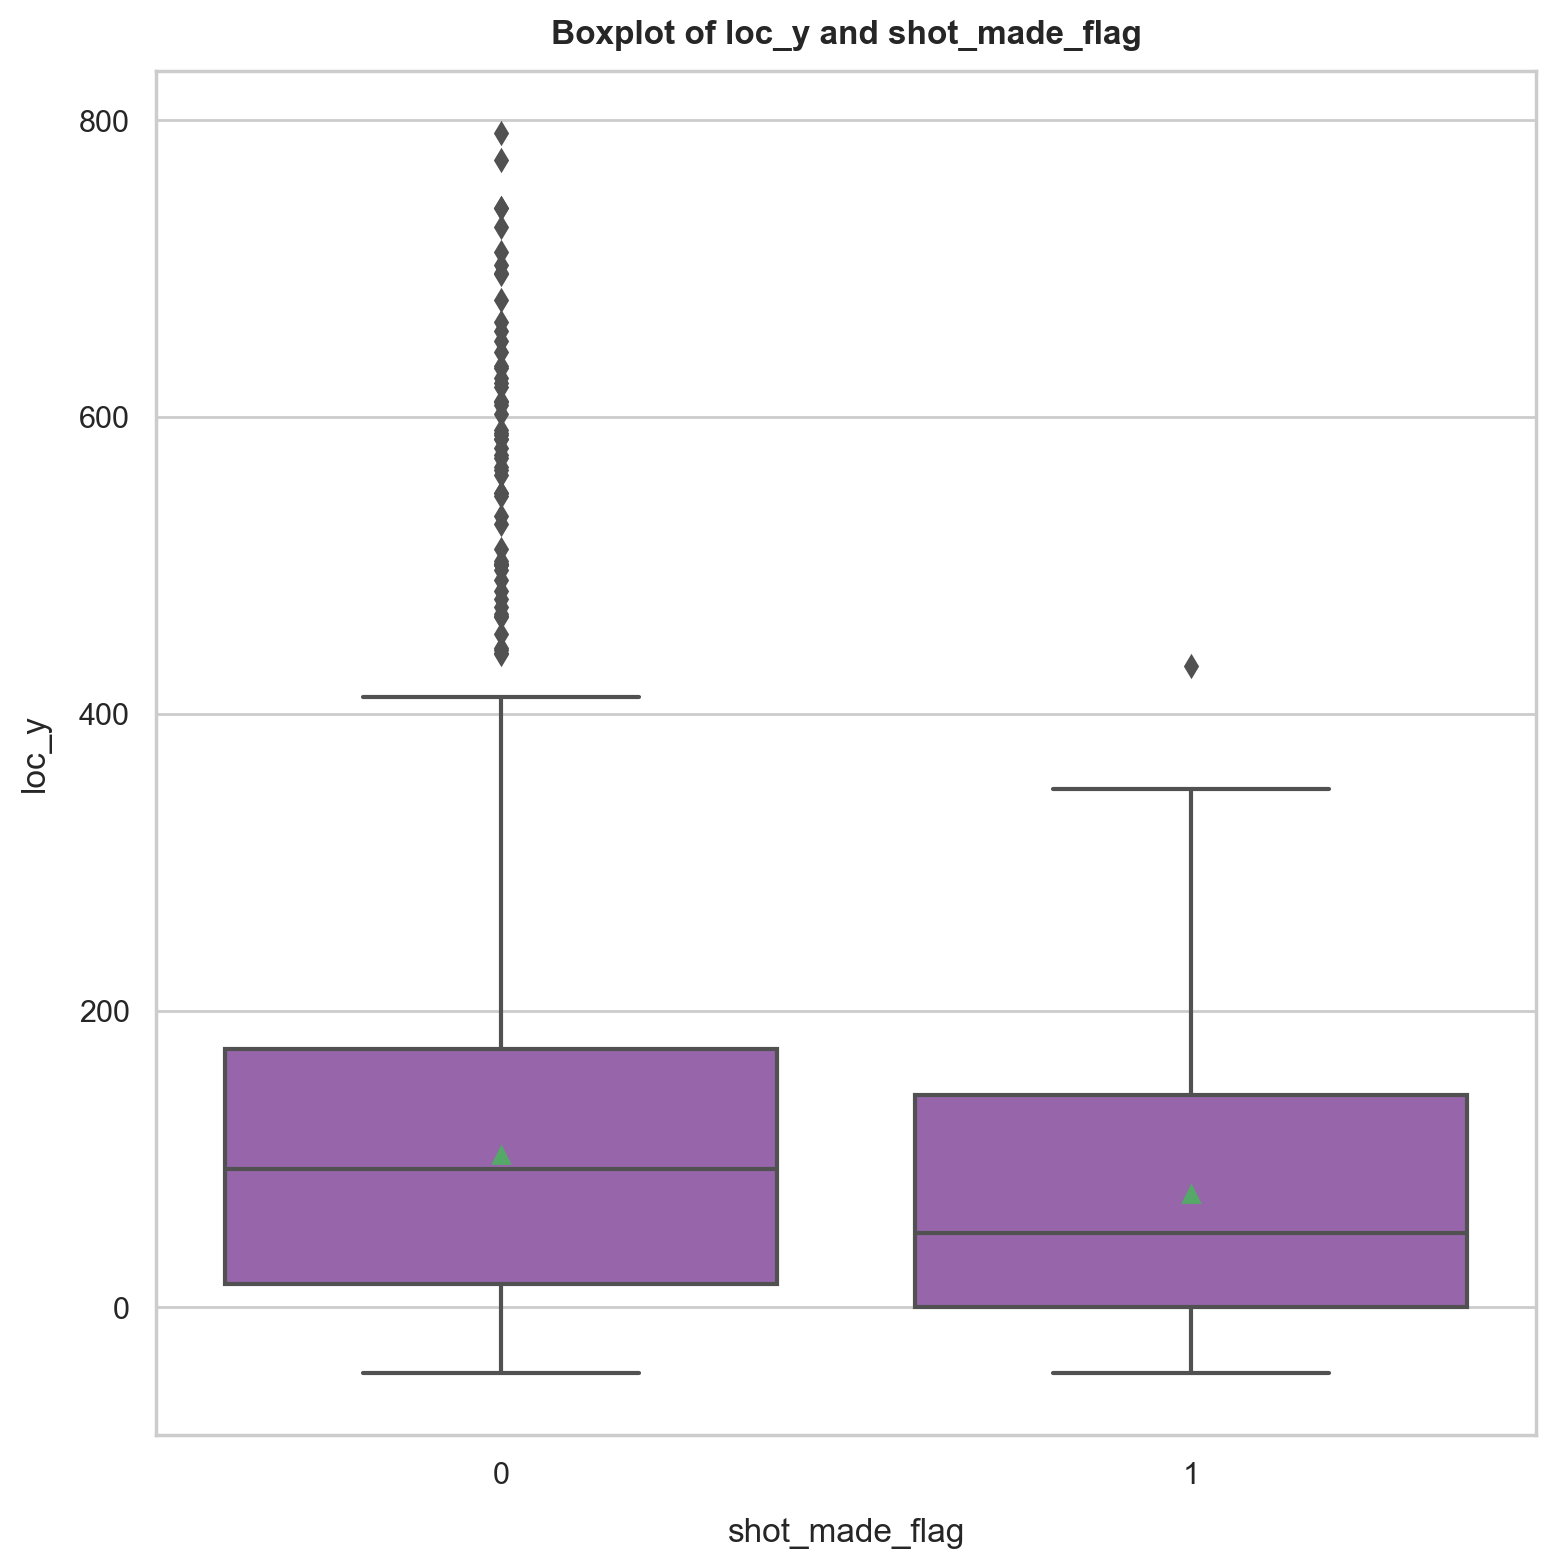
\includegraphics[scale=0.25]{../figs/boxplot_loc_y.png}}
        \caption{\label{fig:boxplot_loc_y} Boxplot of Shot Y Location}
      \label{fig:1}
    \end{subfigure}
    %
    \begin{subfigure}[b]{0.4\textwidth}
        \center{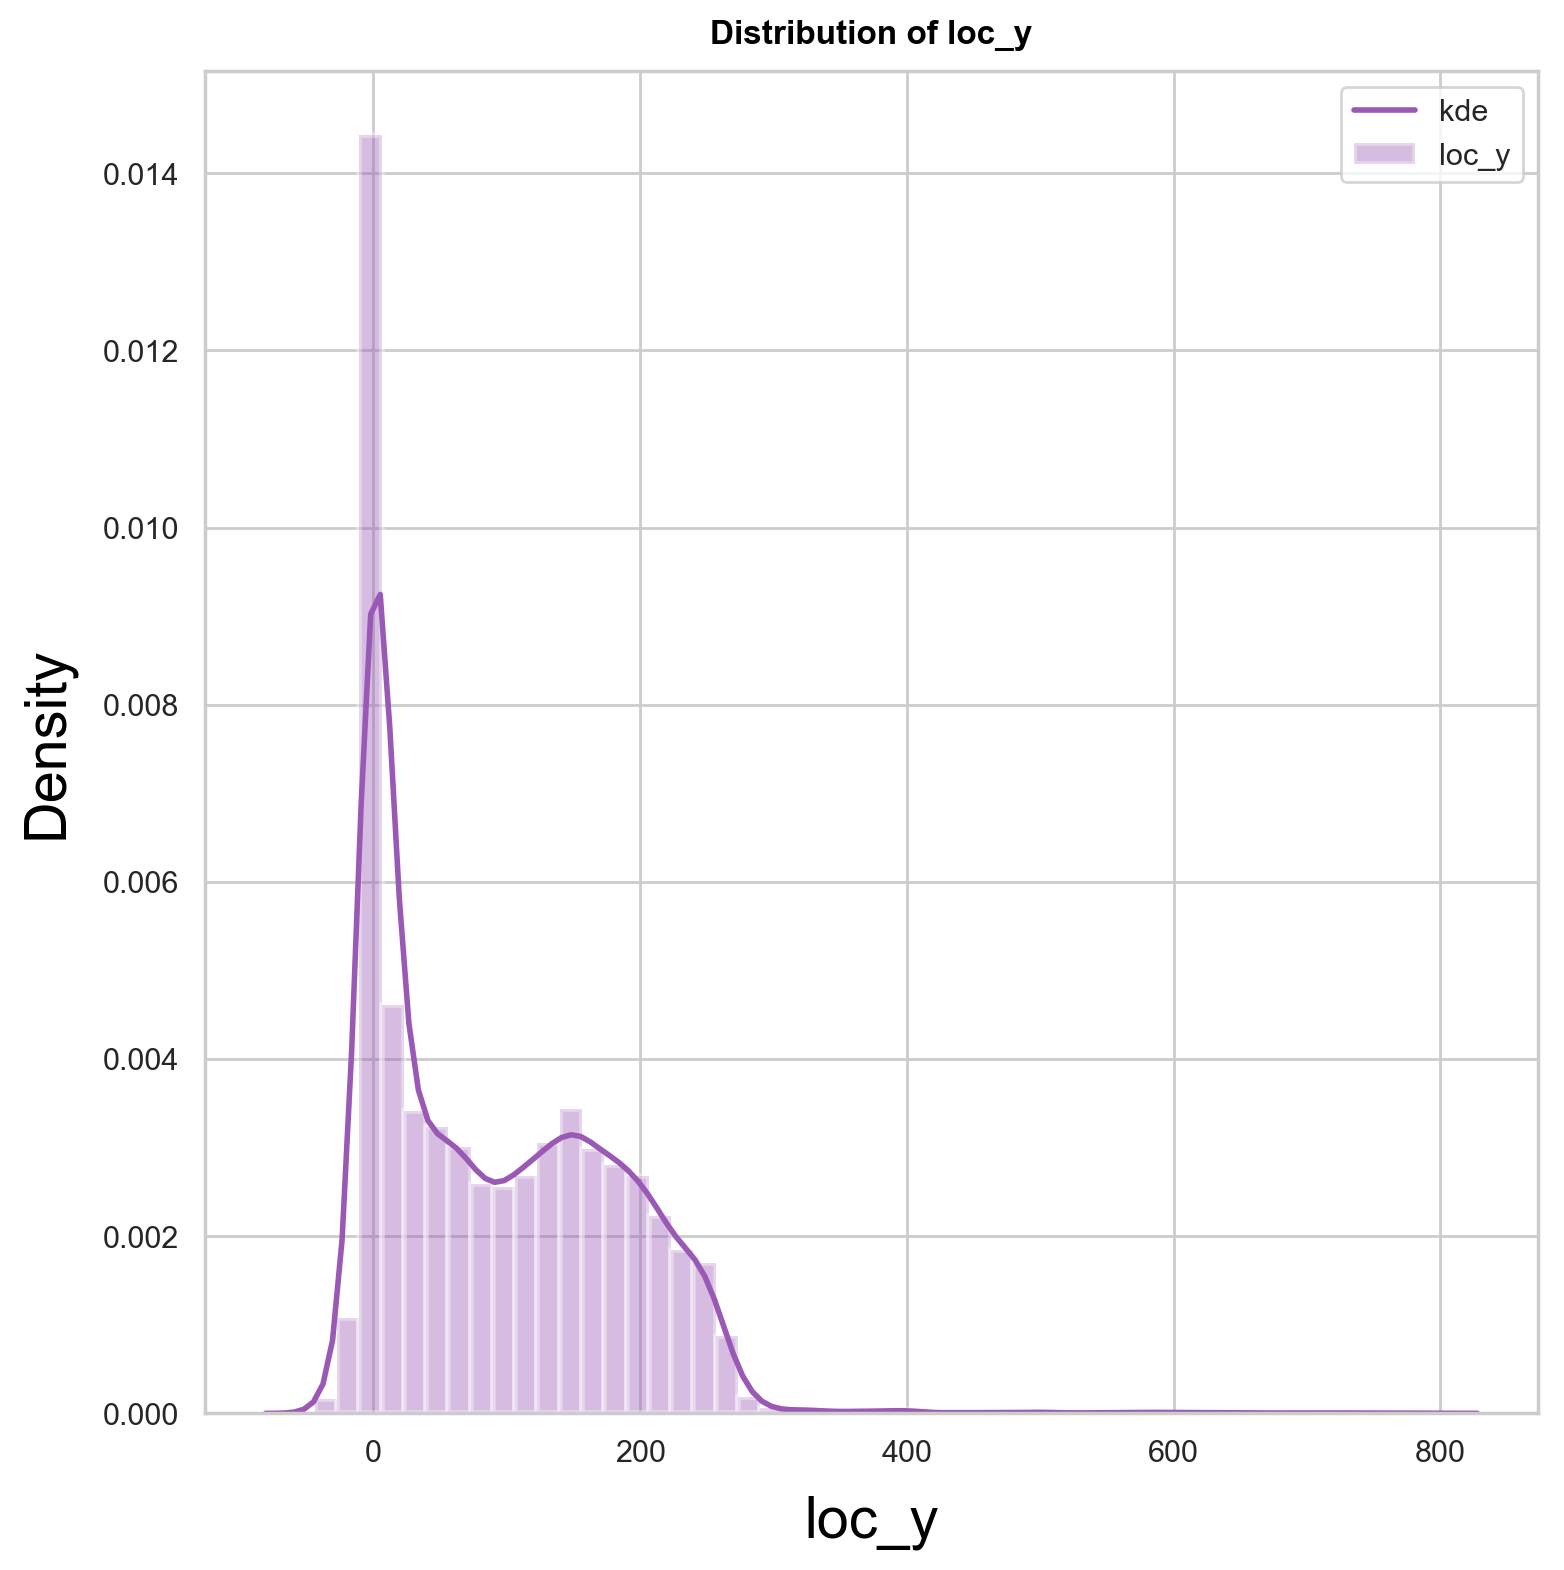
\includegraphics[scale=0.25]{../figs/distplot_loc_y.png}}
        \caption{\label{fig:distplot_loc_y} Distplot of Shot Y Location}
      \label{fig:2}
    \end{subfigure}
    \caption{\label{fig:y_loc_plots} Plots of y\_loc}
  \end{figure}


It's clear that outliers are prevalent in some of the features, particularly those representing the distance to the hoop and the time remaining, as represented in figures \ref{fig:distplot_loc_y} and \ref{fig:boxplot_loc_y}.  Several solutions were explored to mitigate the potential impact of the outliers, none of which yielded a model with better results. Thus, all outliers were included in the final models on their original scale.\par


\begin{figure}[!htb]
    \center{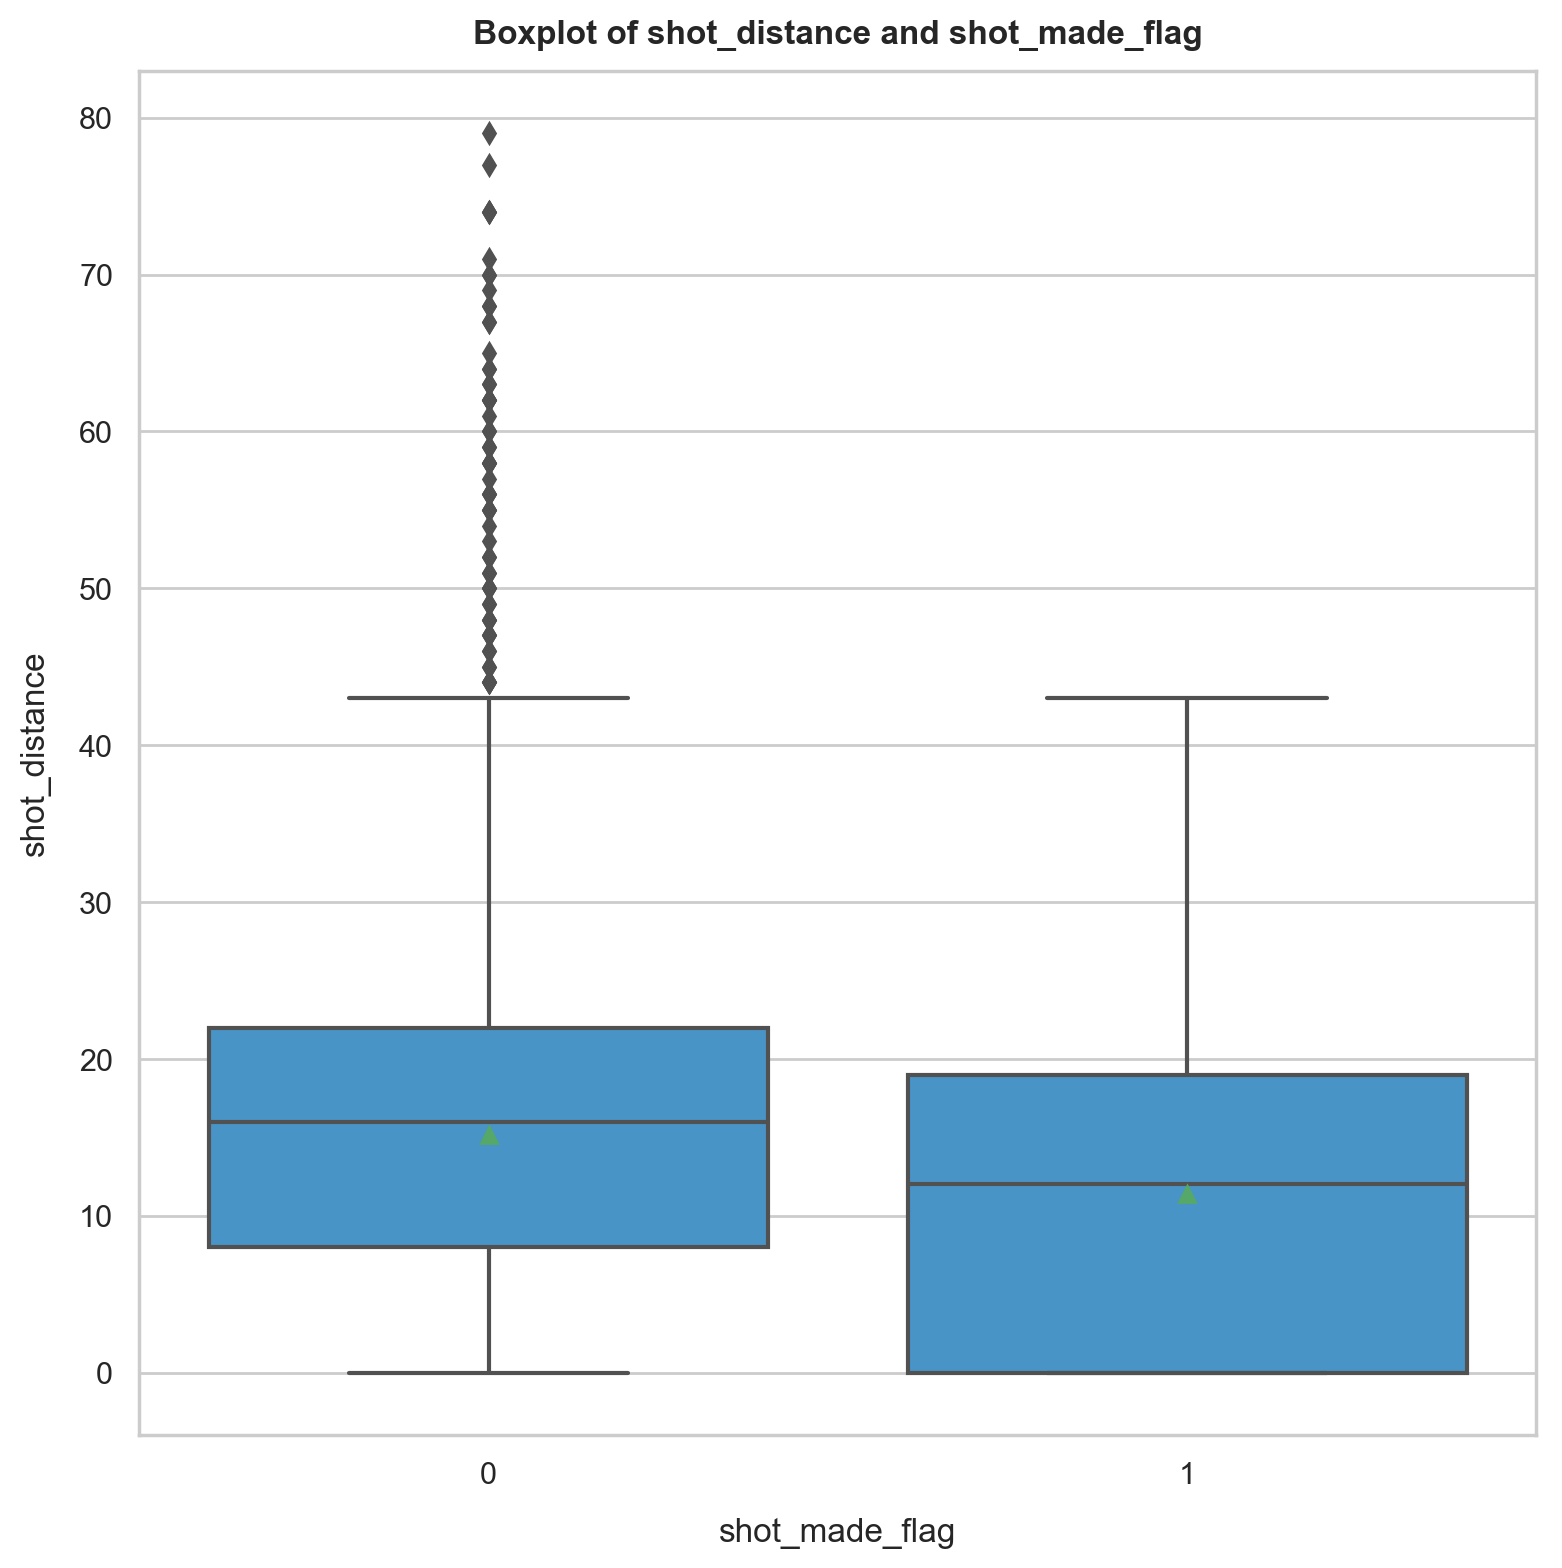
\includegraphics[width=0.5\textwidth]{../figs/boxplot_shot_distance.png}}
    \caption{\label{fig:boxplot_shot_distance} Boxplot of Shot Distance}
\end{figure}


The exploratory boxplot of shot\_distance (figure \ref{fig:boxplot_shot_distance}) already hints at a potential relationship between a shot's likelyhood of being made verses the distance the shot was taken from the hoop.\par



\subsection{Multicollinearity}
The base feature set was wrought with violations of independent variability.  As noted in the table and it's accompanying correlation matrix, approximately half of the features showed a collinear relationship with other features in the data set. This caused our approach to feature selection vary from the normal methods.  We chose to ignore the more nuanced stepwise / LASSO / LarsCV methods and instead implemented a procedure to recursively drop a feature with an exorbitant variance inflation factor on each iteration until reaching a feature set that showed no multicollinearity violations.  We used an elimination cutoff of the initial median VIF + 2 standard deviations.  Variance inflation factors for the original features can be seen in table \ref{tbl:vifs}. A correlation matrix of the same feature set is displayed in figure \ref{fig:corr_matrix_allvars}.


\begin{figure}[!htb]
    \centering
    \center{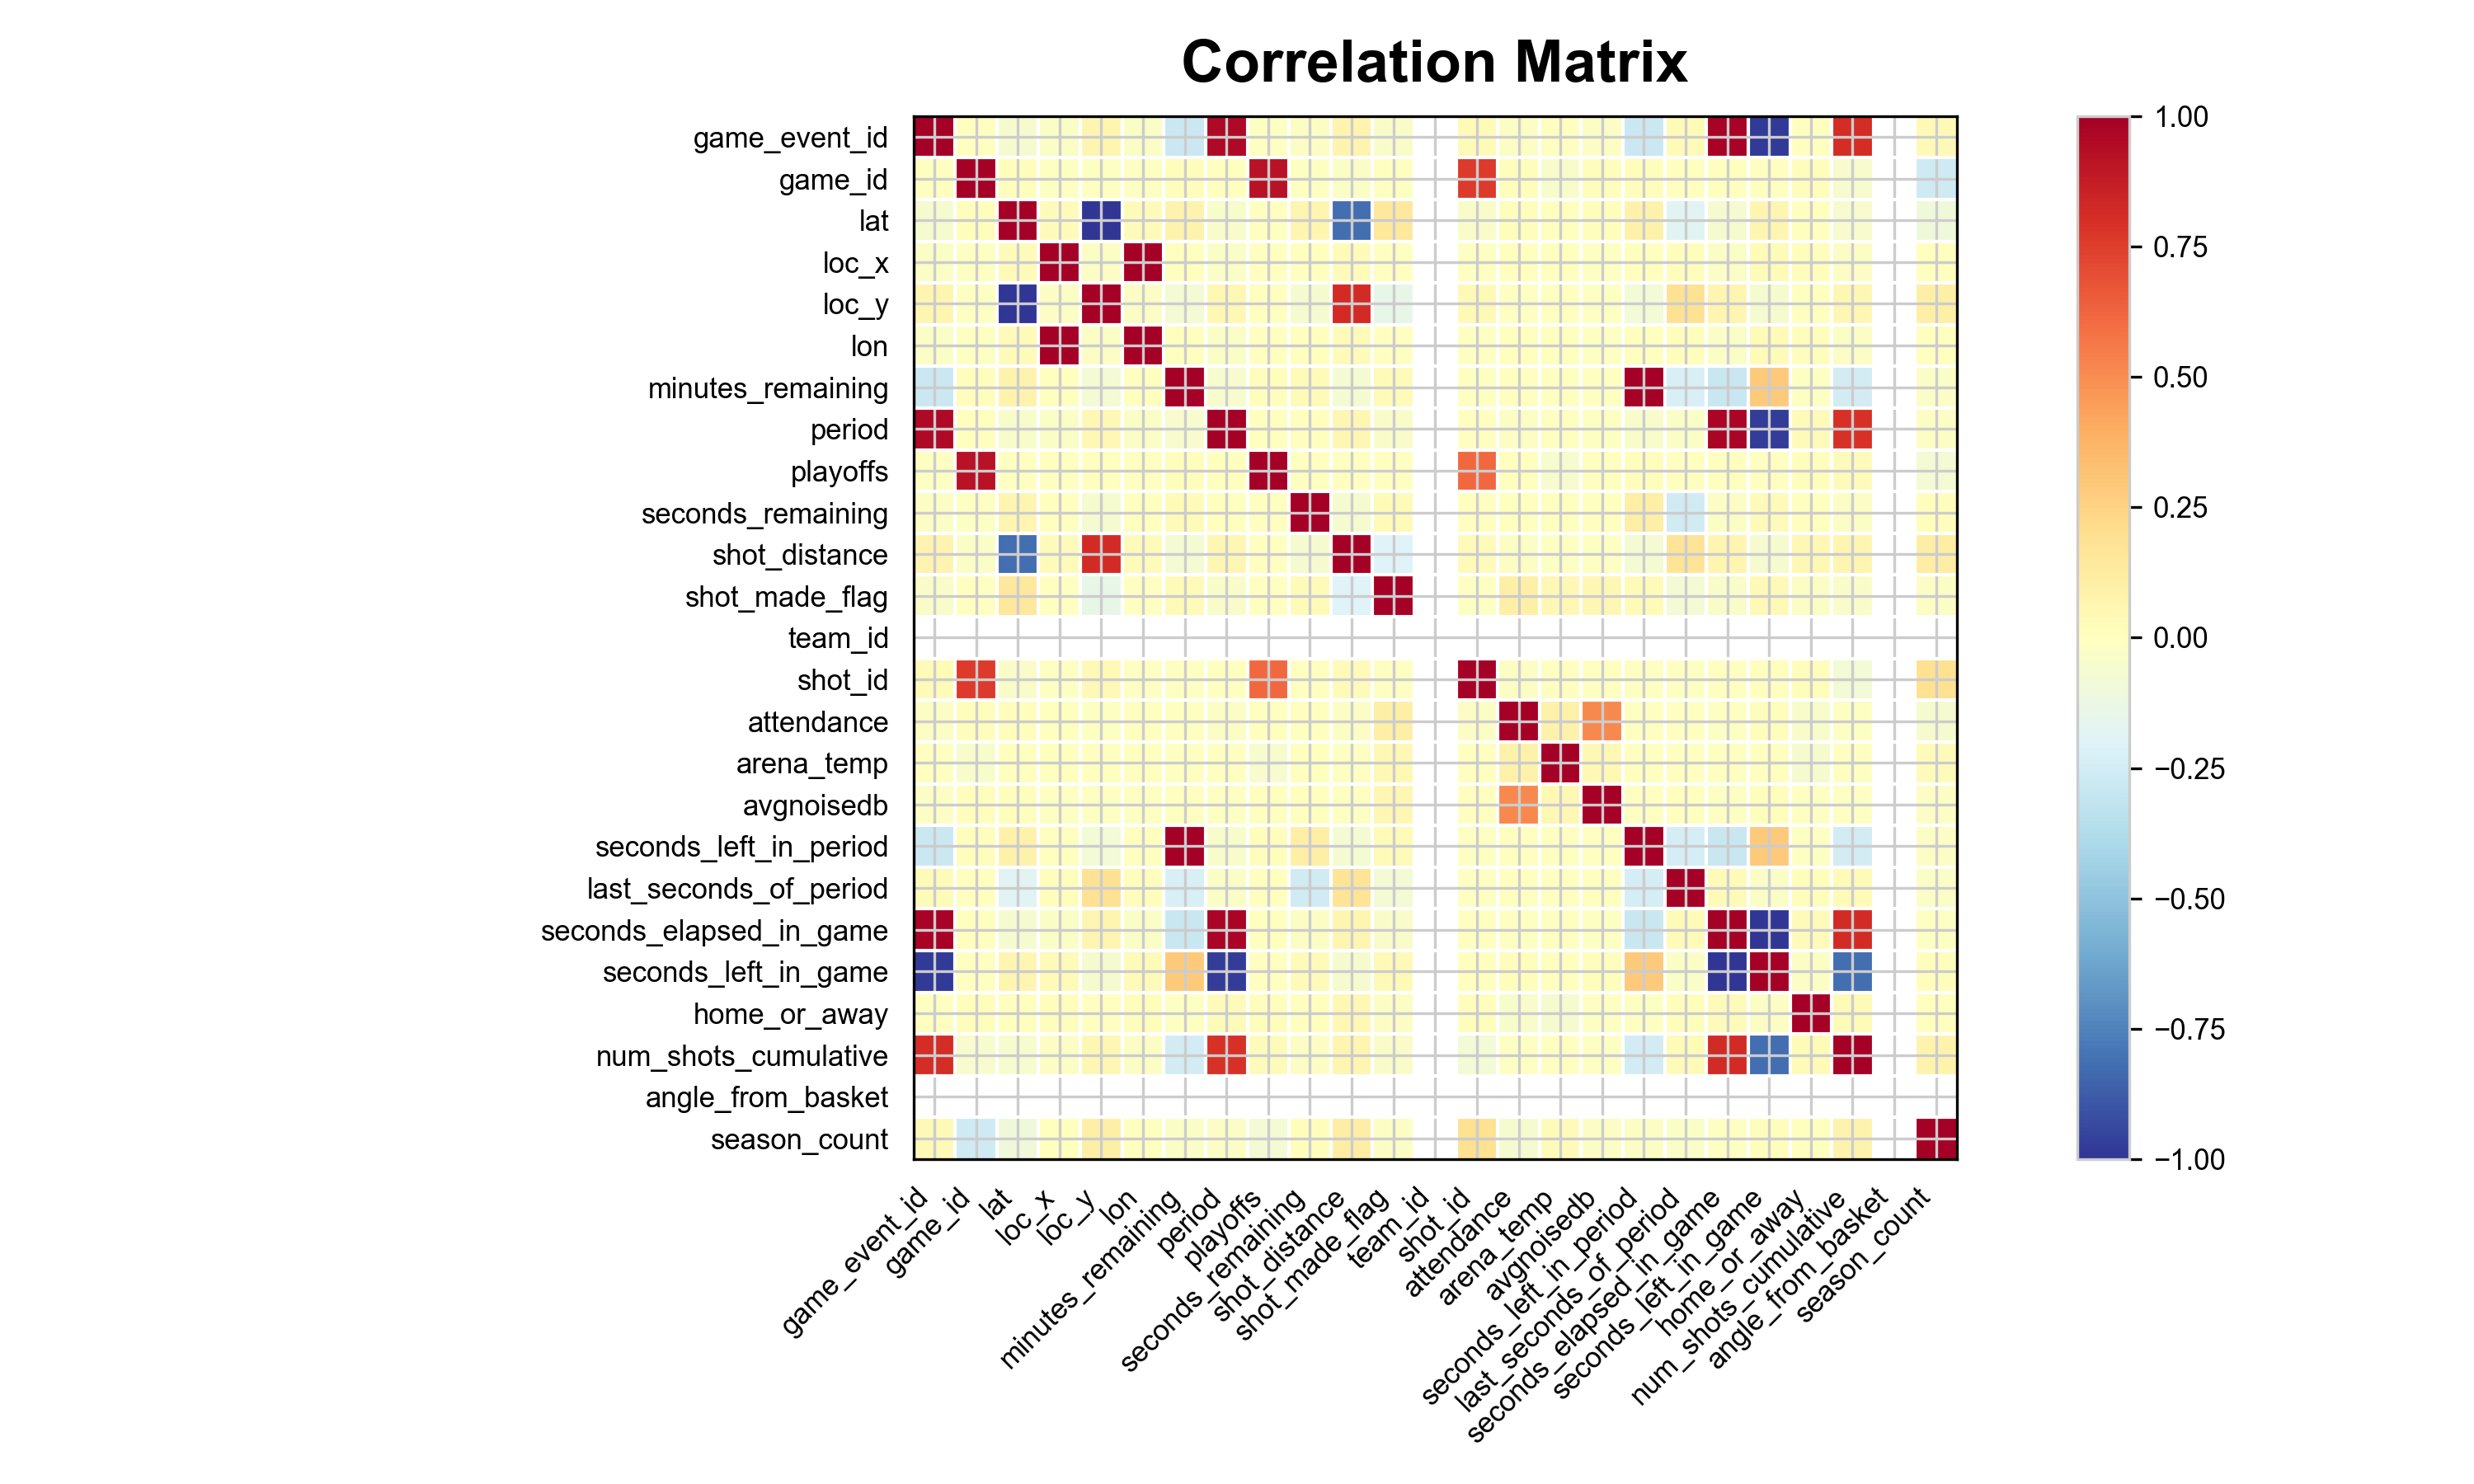
\includegraphics[width=1\textwidth]{../figs/corr_matrix_allvars.png}}
    \caption{\label{fig:corr_matrix_allvars} Correlation Matrix - All features}
\end{figure}
\cite{cm}

\resizebox{.3 \textwidth}{!} {
\begin{tabular}{lrl}
    \toprule
    {} &  VIF Factor &                 features \\
    \midrule
    0  &           0 &                Intercept \\
    1  &          35 &            game\_event\_id \\
    2  &          68 &                  game\_id \\
    3  &         inf &                      lat \\
    4  &         inf &                    loc\_x \\
    5  &         inf &                    loc\_y \\
    6  &         inf &                      lon \\
    7  &         inf &        minutes\_remaining \\
    8  &         inf &                   period \\
    9  &          29 &                 playoffs \\
    10 &         inf &        seconds\_remaining \\
    11 &           3 &            shot\_distance \\
    12 &           0 &                  team\_id \\
    13 &          14 &                  shot\_id \\
    \bottomrule
    \end{tabular}
    }
    \captionof{table}{Variance Inflation Factors}\label{tbl:vifs}

% \subsection{Illustration}
